\documentclass[10pt,letterpaper]{article}
\usepackage[utf8]{inputenc}
\usepackage[T1]{fontenc}
\usepackage[provide=*,spanish]{babel}
\usepackage{lmodern,geometry,amsmath,graphicx,xcolor,microtype,multicol}
\usepackage{caption,fancyhdr,enumitem,booktabs,tabularx,array}
\usepackage{circuitikz,pgfplots,siunitx,hyperref}
\pgfplotsset{compat=1.18}
\usetikzlibrary{arrows.meta}
\geometry{top=1.8cm,bottom=2.0cm,left=1.75cm,right=1.75cm,headheight=14pt}
\setlength{\columnsep}{0.65cm}
\setlength{\parindent}{0pt}
\setlength{\parskip}{0.42em}
\setlist{nosep,leftmargin=*}
\sisetup{output-decimal-marker={,},group-separator={\,},per-mode=symbol}
\DeclareSIUnit{\division}{div}
\captionsetup{font=small,labelfont=bf,justification=centering,skip=4pt,hypcap=false}
\definecolor{udecazul}{HTML}{003A70}
\definecolor{udecoro}{HTML}{C79A2B}
\definecolor{observado}{HTML}{B05D22}
\definecolor{grisedicion}{HTML}{666666}
\addto\captionsspanish{\renewcommand{\tablename}{Tabla}}

% DATOS DE PORTADA: revisar fecha, nombres y sección antes de entregar.
\newcommand{\asignatura}{Electromagnetismo 2}
\newcommand{\laboratorio}{Laboratorio 3}
\newcommand{\tituloinforme}{Desfase entre corriente y voltaje en circuitos RC y RL, y resonancia en un circuito RLC en serie}
\newcommand{\autores}{Nicolás Ruiz, Julio Bastías}
\newcommand{\procedencia}{Departamento de Física, Universidad de Concepción, Chile}
\newcommand{\docente}{Juan Staforelli Vivanco}
\newcommand{\ayudante}{Cristóbal Valdés Cruces, Catalina Gidi Chomalí}
\newcommand{\seccion}{Sección 2}
\newcommand{\fechaentrega}{Fecha por completar}
\hypersetup{colorlinks=true,linkcolor=udecazul,citecolor=udecazul,urlcolor=udecazul,
  pdftitle={Laboratorio 3: Desfase y resonancia},pdfauthor={Nicolas Ruiz y Julio Bastias}}
\pagestyle{fancy}
\fancyhf{}
\lhead{\small \laboratorio: Desfase y resonancia}
\rhead{\small \asignatura}
\cfoot{\small \thepage}
\renewcommand{\headrulewidth}{0.4pt}
\fancypagestyle{plain}{%
 \fancyhf{}
 \lhead{\small \laboratorio: Desfase y resonancia}
 \rhead{\small \asignatura}
 \cfoot{\small \thepage}
 \renewcommand{\headrulewidth}{0.4pt}}
\newcommand{\porcompletar}[1]{\textcolor{grisedicion}{\textit{Por completar: #1}}}
% Parámetros para las gráficas, en unidades indicadas.
% Las tablas y el texto se editan aparte: no se recalculan desde este archivo.
\newcommand{\RRC}{1.6} % kOhm
\newcommand{\CRC}{10} % nF
\newcommand{\RRL}{1.6} % kOhm, supuesto
\newcommand{\LRL}{9} % mH
\newcommand{\RRLC}{1} % kOhm
\newcommand{\LRLC}{9} % mH
\newcommand{\CRLC}{10} % nF
\newcommand{\FDial}{17} % kHz, lectura orientativa
\pgfmathsetmacro{\FRes}{1000/(2*pi*sqrt(\LRLC*\CRLC))}
\newcommand{\PuntosRC}{(0.5,86.735751) (1,89.454545) (8,50.855019)}
\newcommand{\PuntosRL}{(10,-23.376623) (50,-57.525773) (100,-74.226804)}
\newcommand{\FaseRCA}{86.735751}
\newcommand{\FaseRCB}{89.454545}
\newcommand{\FaseRCC}{50.855019}
\newcommand{\FaseRLA}{23.376623}
\newcommand{\FaseRLB}{57.525773}
\newcommand{\FaseRLC}{74.226804}


\begin{document}
\thispagestyle{empty}
\begin{center}
  \begin{minipage}{0.46\textwidth}
    \raggedright
\includegraphics[width=0.68\linewidth]{figuras/logo_udec.png}
  \end{minipage}
  \begin{minipage}{0.46\textwidth}
    \raggedleft
\includegraphics[width=0.68\linewidth]{figuras/logo_fcfm.png}
  \end{minipage}
  {\color{udecoro}\rule{0.82\textwidth}{1.2pt}\par}
  \vspace{0.12cm}
  {\Large\bfseries \asignatura\par}
  \vspace{0.16cm}
  {\large\bfseries\color{udecazul} \laboratorio\par}
  \vspace{0.10cm}
  {\Large\bfseries\color{udecazul} \tituloinforme\par}
  \vspace{0.12cm}
  {\normalsize Informe experimental\par}
  \vspace{0.12cm}
  {\small \autores\par}
  {\footnotesize\itshape \procedencia\par}
  \vspace{0.06cm}
  {\small Docente: \docente\par}
  {\small Ayudantes: \ayudante\par}
  {\small \seccion \quad $\vert$ \quad \fechaentrega\par}
\end{center}

\begin{abstract}
Se estudió la diferencia de fase entre la corriente y el voltaje aplicado en circuitos RC y RL, y la condición de resonancia de un circuito RLC en serie. Se compararon las señales del generador y del resistor mediante un osciloscopio de dos canales. En RC se obtuvieron magnitudes de desfase de \SI{86.7}{\degree}, \SI{89.5}{\degree} y \SI{50.9}{\degree} para frecuencias nominales de \SI{500}{\hertz}, \SI{1}{\kilo\hertz} y \SI{8}{\kilo\hertz}; en RL se estimaron \SI{23.4}{\degree}, \SI{57.5}{\degree} y \SI{74.2}{\degree} a \SI{10}{\kilo\hertz}, \SI{50}{\kilo\hertz} y \SI{100}{\kilo\hertz}. Las diferencias con el modelo ideal no superaron aproximadamente \SI{5.2}{\degree}. Los tiempos se reconstruyeron a partir de las frecuencias nominales, mientras que el desfase se obtuvo directamente del cociente entre distancias de la pantalla. Para RLC, la frecuencia teórica fue \SI{16.8}{\kilo\hertz}, cercana a una lectura orientativa del generador de \SI{17}{\kilo\hertz}. Los resultados reproducen las tendencias previstas, con las limitaciones del registro fotográfico disponible.
\end{abstract}

\begin{multicols}{2}
\raggedcolumns
\section{Introducción}
En corriente alterna, un condensador y una bobina modifican tanto la amplitud como la fase de la corriente. En un circuito RC la corriente adelanta al voltaje aplicado, mientras que en un circuito RL se retrasa. En un circuito RLC en serie, ambos efectos pueden compensarse y dar lugar a la resonancia \cite{young2009}.

Esta experiencia siguió la guía del Laboratorio 3 \cite{guia2026}. Se utilizaron las dos señales del osciloscopio para obtener el desfase de la corriente respecto del generador y comparar su variación con la frecuencia. Además, se examinó la proximidad a la resonancia en el montaje RLC.

\section{Objetivos}
Medir y comparar con el modelo ideal el adelanto de la corriente en RC y su retraso en RL para las frecuencias indicadas en la guía. Reconocer la condición de resonancia de un circuito RLC en serie y relacionarla con sus diagramas de fasores.

\section{Marco teórico}
\subsection{Señales y medición de fase}
En un resistor ideal, el voltaje $v_R(t)$ está en fase con la corriente $i(t)$, puesto que
\begin{equation}
  v_R(t)=R\,i(t).
\end{equation}
Por ello, comparar $v_R(t)$ con el voltaje del generador $v_g(t)$ permite estudiar el desfase de la corriente. Si $\Delta h$ es la separación horizontal de puntos equivalentes de ambas ondas y $H$ la distancia de un período de una misma señal, ambas en divisiones, entonces
\begin{equation}
  |\Delta\varphi|=2\pi\frac{\Delta t}{T}=2\pi\frac{\Delta h}{H}.
  \label{eq:fase}
\end{equation}
Aquí $\Delta t$ es la separación temporal y $T$ el período. El cociente determina la magnitud del ángulo; el orden de las señales determina quién adelanta a quién \cite{manualhameg}.

\subsection{Reactancias y fasores}
Para frecuencia $f$ y frecuencia angular $\omega=2\pi f$, las reactancias inductiva y capacitiva son
\begin{equation}
  X_L=\omega L,\qquad X_C=\frac{1}{\omega C}.
  \label{eq:reactancias}
\end{equation}
Tomando la corriente como referencia horizontal, $\widetilde V_R$ está en fase con ella, $\widetilde V_L$ adelanta \SI{90}{\degree} y $\widetilde V_C$ se retrasa \SI{90}{\degree}. El voltaje aplicado es la suma de estos fasores \cite{young2009}.

\subsection{Circuitos RC y RL}
Las impedancias ideales son $Z_{RC}=R-jX_C$ y $Z_{RL}=R+jX_L$, donde $j^2=-1$. La fase de la corriente respecto del generador, $\psi=\arg\widetilde I-\arg\widetilde V_g$, resulta
\begin{align}
 \psi_{RC}&=+\arctan\!\left(\frac{1}{\omega RC}\right),\label{eq:rc}\\
 \psi_{RL}&=-\arctan\!\left(\frac{\omega L}{R}\right).\label{eq:rl}
\end{align}
El signo positivo indica adelanto y el negativo, retraso. Las tablas presentan la magnitud $|\Delta\varphi|=|\psi|$ y describen el sentido por separado.

\subsection{Resonancia en RLC}
En serie, $Z=R+j(X_L-X_C)$. La fase del voltaje aplicado respecto de la corriente es
\begin{equation}
  \varphi_V=\arctan\!\left(\frac{\omega L-1/(\omega C)}{R}\right).
  \label{eq:rlc}
\end{equation}
Esta convención tiene signo opuesto a $\psi$. En resonancia $X_L=X_C$, de modo que
\begin{equation}
  f_r=\frac{1}{2\pi\sqrt{LC}}.
  \label{eq:resonancia}
\end{equation}
En el modelo ideal, $\varphi_V=0$, la corriente y el generador están en fase y $\widetilde V_g=\widetilde V_R$. Para $f<f_r$ predomina el comportamiento capacitivo y para $f>f_r$, el inductivo.

\section{Materiales}
\begin{itemize}
 \item Generador de señales senoidales, modelo 062.101.
 \item Osciloscopio de dos canales Hameg HM203-7 y dos puntas de prueba.
 \item Cajas de resistencias y condensadores.
 \item Bobina de 600 vueltas, $L=\SI{9}{\milli\henry}$ nominal.
 \item Cables de conexión.
\end{itemize}
Para RC se emplean los valores nominales de la guía: $R=\SI{1.6}{\kilo\ohm}$ y $C=\SI{0.01}{\micro\farad}$. Para el análisis RL se supone la misma resistencia. En RLC la guía indica $R=\SI{1}{\kilo\ohm}$, $C=\SI{0.01}{\micro\farad}$ y $L=\SI{9}{\milli\henry}$ \cite{guia2026}.
% REVISAR: R de RL se supone igual a RC; cambiar si se dispone de otro registro.

\section{Montaje y procedimiento}
Los esquemas de la figura~\ref{fig:montajes} representan las conexiones de referencia. CH1 registra el generador y CH2 el voltaje del resistor. Ambos canales comparten el nodo de referencia del circuito; el resistor permite representar la fase de la corriente.

Se realizaron dos registros por condición. En RC se consideraron \SI{500}{\hertz}, \SI{1}{\kilo\hertz} y \SI{8}{\kilo\hertz}; en RL, \SI{10}{\kilo\hertz}, \SI{50}{\kilo\hertz} y \SI{100}{\kilo\hertz}. Se fotografiaron las señales y la escala de tiempo, y se eligieron los tramos donde ambas trazas podían distinguirse. Se estimaron $H$ y $\Delta h$ con corrección de perspectiva y se aplicó la ecuación~\eqref{eq:fase}.

Para RLC se varió la frecuencia buscando la mayor coincidencia de fase entre las señales. El registro conservado permite describir la proximidad a esa condición y estimar la frecuencia mediante el dial del generador.
\end{multicols}

\begin{center}
 \begin{minipage}[t]{0.31\textwidth}
\centering
\resizebox{\linewidth}{!}{%
\begin{circuitikz}[american]
 \draw (0,0) to[sV,l=$v_g$] (0,3)
  to[C,l=$C$,i>^=$i$] (3,3) to[R] (3,0) -- (0,0);
 \draw (0,3) node[circ]{} node[above left]{CH1};
 \draw (3,3) node[circ]{} node[above right]{CH2};
 \draw (1.5,0) node[ground]{};
 \node[left] at (2.7,1.5) {$R$};
 \node[right] at (3.3,1.5) {$v_R$};
\end{circuitikz}}
\par\small (a) RC.
\end{minipage}\hfill
\begin{minipage}[t]{0.31\textwidth}
\centering
\resizebox{\linewidth}{!}{%
\begin{circuitikz}[american]
 \draw (0,0) to[sV,l=$v_g$] (0,3)
  to[L,l=$L$,i>^=$i$] (3,3) to[R] (3,0) -- (0,0);
 \draw (0,3) node[circ]{} node[above left]{CH1};
 \draw (3,3) node[circ]{} node[above right]{CH2};
 \draw (1.5,0) node[ground]{};
 \node[left] at (2.7,1.5) {$R$};
 \node[right] at (3.3,1.5) {$v_R$};
\end{circuitikz}}
\par\small (b) RL.
\end{minipage}\hfill
\begin{minipage}[t]{0.33\textwidth}
\centering
\resizebox{\linewidth}{!}{%
\begin{circuitikz}[american]
 \draw (0,0) to[sV,l=$v_g$] (0,3)
  to[L,l=$L$,i>^=$i$] (2,3) to[C,l=$C$] (4,3)
  to[R] (4,0) -- (0,0);
 \draw (0,3) node[circ]{} node[above left]{CH1};
 \draw (4,3) node[circ]{} node[above right]{CH2};
 \draw (2,0) node[ground]{};
 \node[left] at (3.7,1.5) {$R$};
 \node[right] at (4.3,1.5) {$v_R$};
\end{circuitikz}}
\par\small (c) RLC en serie.
\end{minipage}

 \captionof{figure}{Esquemas de referencia de los circuitos RC, RL y RLC en serie. Se indica la medición de $v_g$ con CH1 y de $v_R$ con CH2; los diagramas describen la conexión eléctrica y no la disposición física de los componentes.}
 \label{fig:montajes}
\end{center}

\section{Resultados}
\subsection{Reconstrucción de los tiempos}
Las tablas~\ref{tab:rc} y \ref{tab:rl} siguen las columnas solicitadas en la guía. Se supone que la frecuencia nominal $f$ es correcta y se reconstruye el factor de tiempo efectivo mediante
\begin{equation}
 T_{\mathrm{est}}=\frac{1}{f},\qquad
 f_{h,\mathrm{est}}=\frac{1}{fH},\qquad
 \Delta t_{\mathrm{est}}=\frac{\Delta h}{fH}.
 \label{eq:reconstruccion}
\end{equation}
\textbf{Estos tiempos son estimaciones a partir de la frecuencia nominal.} El valor $f_{h,\mathrm{est}}$ no es una lectura calibrada del selector TIME/DIV. El ángulo sigue siendo el obtenido de la foto mediante $\Delta h/H$.

\begin{table}[htbp]
\centering
\footnotesize
\setlength{\tabcolsep}{4pt}
\caption{Circuito RC: la corriente adelanta a $v_g$. Lecturas fotográficas, tiempos estimados y comparación con el modelo ideal.}
\label{tab:rc}
\begin{tabular}{ccccccccc}
\toprule
\shortstack{$f$\\(Hz)} &
\shortstack{$\Delta h$\\(div)} &
\shortstack{$H$\\(div)} &
\shortstack{$f_{h,\mathrm{est}}$\\(s/div)} &
\shortstack{$\Delta t_{\mathrm{est}}$\\(s)} &
\shortstack{$T_{\mathrm{est}}$\\(s)} &
\shortstack{$|\Delta\varphi|_{\mathrm{foto}}$\\(rad; grados)} &
\shortstack{$|\psi|_{\mathrm{teo}}$\\(grados)} &
\shortstack{$\delta$\\(grados)} \\
\midrule
500 & \num{0.465} & \num{1.93} &
\num{1.04e-3} & \num{4.82e-4} &
\num{2.00e-3} & \num{1.51}; \num{86.7} &
\num{87.1} & \num{-0.4} \\

1000 & \num{0.41} & \num{1.65} &
\num{6.06e-4} & \num{2.48e-4} &
\num{1.00e-3} & \num{1.56}; \num{89.5} &
\num{84.3} & \num{5.2} \\

8000 & \num{0.38} & \num{2.69} &
\num{4.65e-5} & \num{1.77e-5} &
\num{1.25e-4} & \num{0.89}; \num{50.9} &
\num{51.2} & \num{-0.3} \\
\bottomrule
\end{tabular}
\end{table}


\begin{table}[htbp]
\centering
\footnotesize
\setlength{\tabcolsep}{4pt}
\caption{Circuito RL: la corriente se retrasa respecto de $v_g$. Lecturas fotográficas, tiempos estimados y comparación con el modelo ideal.}
\label{tab:rl}
\begin{tabular}{ccccccccc}
\toprule
\shortstack{$f$\\(kHz)} &
\shortstack{$\Delta h$\\(div)} &
\shortstack{$H$\\(div)} &
\shortstack{$f_{h,\mathrm{est}}$\\(s/div)} &
\shortstack{$\Delta t_{\mathrm{est}}$\\(s)} &
\shortstack{$T_{\mathrm{est}}$\\(s)} &
\shortstack{$|\Delta\varphi|_{\mathrm{foto}}$\\(rad; grados)} &
\shortstack{$|\psi|_{\mathrm{teo}}$\\(grados)} &
\shortstack{$\delta$\\(grados)} \\
\midrule
10 & \num{0.10} & \num{1.54} &
\num{6.49e-5} & \num{6.49e-6} &
\num{1.00e-4} & \num{0.41}; \num{23.4} &
\num{19.5} & \num{3.9} \\

50 & \num{0.31} & \num{1.94} &
\num{1.03e-5} & \num{3.20e-6} &
\num{2.00e-5} & \num{1.00}; \num{57.5} &
\num{60.5} & \num{-3.0} \\

100 & \num{0.20} & \num{0.97} &
\num{1.03e-5} & \num{2.06e-6} &
\num{1.00e-5} & \num{1.30}; \num{74.2} &
\num{74.2} & \num{0.0} \\
\bottomrule
\end{tabular}
\end{table}



\subsection{Comparación con el modelo ideal}
La tabla~\ref{tab:comparacion} compara las magnitudes de fase con las ecuaciones~\eqref{eq:rc} y \eqref{eq:rl}. La diferencia se expresa en grados como valor fotográfico menos valor teórico. La figura~\ref{fig:fase_rc_rl} incorpora el sentido del desfase de la corriente: positivo para RC y negativo para RL.
\begin{table}[htbp]
\centering
\small
\setlength{\tabcolsep}{6pt}
\caption{Comparación angular con el modelo ideal, usando los componentes nominales.}
\label{tab:comparacion}
\begin{tabular}{ccccc}
\toprule
Circuito & $f$ (Hz) & $|\Delta\varphi|_{\mathrm{foto}}$ (°) & $|\Delta\varphi|_{\mathrm{teo}}$ (°) & Foto $-$ teoría (°) \\
\midrule
RC & 500 & \num{86.7} & \num{87.1} & \num{-0.4} \\
RC & 1000 & \num{89.5} & \num{84.3} & \num{5.2} \\
RC & 8000 & \num{50.9} & \num{51.2} & \num{-0.3} \\
RL & 10000 & \num{23.4} & \num{19.5} & \num{3.9} \\
RL & 50000 & \num{57.5} & \num{60.5} & \num{-3.0} \\
RL & 100000 & \num{74.2} & \num{74.2} & \num{0.0} \\
\bottomrule
\end{tabular}
\end{table}

\begin{center}
 \begin{minipage}{0.49\textwidth}
\centering
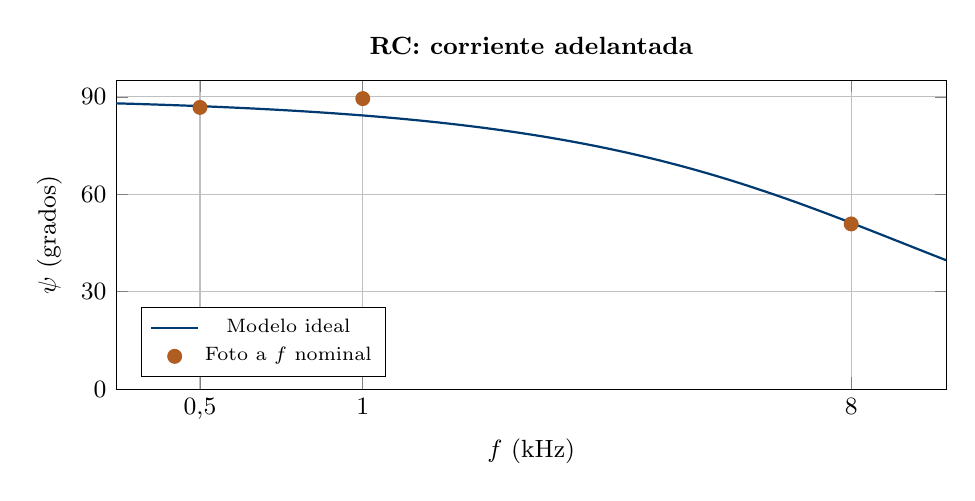
\begin{tikzpicture}
\begin{axis}[width=\linewidth,height=5.5cm,xmode=log,xmin=0.35,xmax=12,ymin=0,ymax=95,
 xlabel={$f$ (kHz)},ylabel={$\psi$ (grados)},title={RC: corriente adelantada},
 xtick={0.5,1,8},xticklabels={$0{,}5$,$1$,$8$},ytick={0,30,60,90},grid=major,
 tick label style={font=\small},label style={font=\small},title style={font=\small\bfseries},
 legend style={font=\scriptsize,at={(0.03,0.04)},anchor=south west}]
 \addplot[udecazul,thick,domain=0.35:12,samples=120]{atan(1000/(2*pi*x*\RRC*\CRC))};
 \addlegendentry{Modelo ideal}
 \addplot[observado,only marks,mark=*,mark size=2.5pt] coordinates {\PuntosRC};
 \addlegendentry{Foto a $f$ nominal}
\end{axis}
\end{tikzpicture}
\end{minipage}\hfill
\begin{minipage}{0.49\textwidth}
\centering
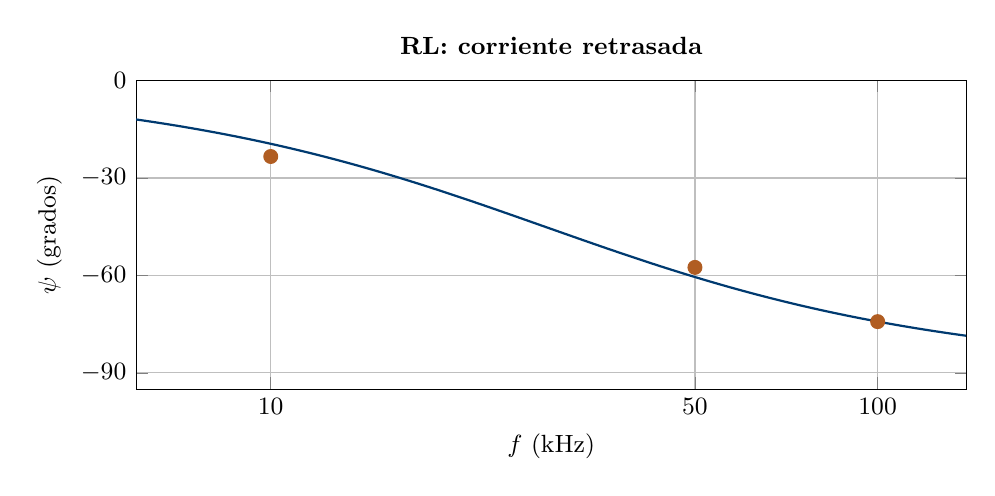
\begin{tikzpicture}
\begin{axis}[width=\linewidth,height=5.5cm,xmode=log,xmin=6,xmax=140,ymin=-95,ymax=0,
 xlabel={$f$ (kHz)},ylabel={$\psi$ (grados)},title={RL: corriente retrasada},
 xtick={10,50,100},xticklabels={$10$,$50$,$100$},ytick={-90,-60,-30,0},grid=major,
 tick label style={font=\small},label style={font=\small},title style={font=\small\bfseries}]
 \addplot[udecazul,thick,domain=6:140,samples=120]{-atan(2*pi*x*\LRL/(1000*\RRL))};
 \addplot[observado,only marks,mark=*,mark size=2.5pt] coordinates {\PuntosRL};
\end{axis}
\end{tikzpicture}
\end{minipage}

 \captionof{figure}{Fase de la corriente respecto del generador. Las curvas representan el modelo ideal y los puntos, las estimaciones fotográficas en las frecuencias nominales; no se asignan barras de incertidumbre sin una caracterización instrumental.}
 \label{fig:fase_rc_rl}
\end{center}

\subsection{Diagramas de fasores de RC y RL}
La figura~\ref{fig:fasores_rc_rl} toma la corriente como referencia horizontal y representa las fases obtenidas de las fotografías. Se normaliza $|\widetilde V_g|=1$, por lo que $V_R=\cos|\psi|$ y $V_X=\sin|\psi|$ son construcciones geométricas del modelo. \textbf{Las longitudes no corresponden a voltajes medidos}; permiten visualizar el adelanto o retraso a partir del ángulo estimado.
\begin{center}
 \begingroup
\newcommand{\panelFasor}[5]{%
 \begin{scope}[shift={(#1,#2)}]
  \pgfmathsetmacro{\xx}{cos(#3)}
  \pgfmathsetmacro{\yy}{sin(#3)}
  \pgfmathsetmacro{\aa}{abs(#3)}
  \draw[-{Stealth[length=2mm]},gray] (0,0) -- (1.25,0) node[right,font=\scriptsize] {$\widetilde I$};
  \draw[-{Stealth[length=2mm]},udecazul,thick] (0,0) -- (\xx,0);
  \node[below,font=\scriptsize,text=udecazul] at (0.32,0) {$\widetilde V_R$};
  \draw[-{Stealth[length=2mm]},udecazul,thick] (0,0) -- (0,\yy) node[left,font=\scriptsize] {$\widetilde V_{#5}$};
  \draw[gray,densely dashed] (\xx,0)--(\xx,\yy)--(0,\yy);
  \draw[-{Stealth[length=2mm]},observado,very thick] (0,0)--(\xx,\yy) node[right,font=\scriptsize] {$\widetilde V_g$};
  \node[font=\small\bfseries] at (0.6,1.45) {#4};
  \node[font=\scriptsize] at (0.6,-1.35) {$|\psi|=\pgfmathprintnumber[fixed,precision=1,use comma]{\aa}^{\circ}$};
 \end{scope}}
\begin{tikzpicture}[x=1.7cm,y=1.5cm]
 \panelFasor{0}{0}{-\FaseRCA}{RC: 500 Hz}{C}
 \panelFasor{3.25}{0}{-\FaseRCB}{RC: 1 kHz}{C}
 \panelFasor{6.5}{0}{-\FaseRCC}{RC: 8 kHz}{C}
 \panelFasor{0}{-3.2}{\FaseRLA}{RL: 10 kHz}{L}
 \panelFasor{3.25}{-3.2}{\FaseRLB}{RL: 50 kHz}{L}
 \panelFasor{6.5}{-3.2}{\FaseRLC}{RL: 100 kHz}{L}
\end{tikzpicture}
\endgroup

 \captionof{figure}{Fasores normalizados construidos con las fases fotográficas. En RC, $\widetilde V_g=\widetilde V_R+\widetilde V_C$ queda bajo la referencia de corriente; en RL, $\widetilde V_g=\widetilde V_R+\widetilde V_L$ queda sobre ella.}
 \label{fig:fasores_rc_rl}
\end{center}

\subsection{Resonancia en RLC}
Con $L=\SI{9e-3}{\henry}$ y $C=\SI{1e-8}{\farad}$, la ecuación~\eqref{eq:resonancia} da $f_r=\SI{16.8}{\kilo\hertz}$. La fotografía del generador muestra el rango de \SI{10}{\kilo\hertz} y un dial situado aproximadamente en 1,7, de donde se obtiene una lectura orientativa de \SI{17}{\kilo\hertz}. La pantalla muestra señales cercanas en fase, con una separación residual visible. No se asigna un desfase exactamente nulo ni una igualdad de voltajes a partir de esa foto.
\begin{table}[htbp]
\centering
\small
\setlength{\tabcolsep}{6pt}
\caption{Resonancia: cálculo nominal y lectura orientativa del dial del generador.}
\label{tab:rlc}
\begin{tabular}{ccccc}
\toprule
$R$ (k$\Omega$) & $L$ (mH) & $C$ ($\mu$F) & $f_{r,\mathrm{teo}}$ (kHz) & $f_{\mathrm{dial}}$ (kHz) \\
\midrule
1 & 9 & \num{0.01} & \num{16.8} & $\approx 17$ \\
\bottomrule
\end{tabular}
\end{table}

\begin{center}
 \begin{minipage}[t]{0.49\textwidth}
  \centering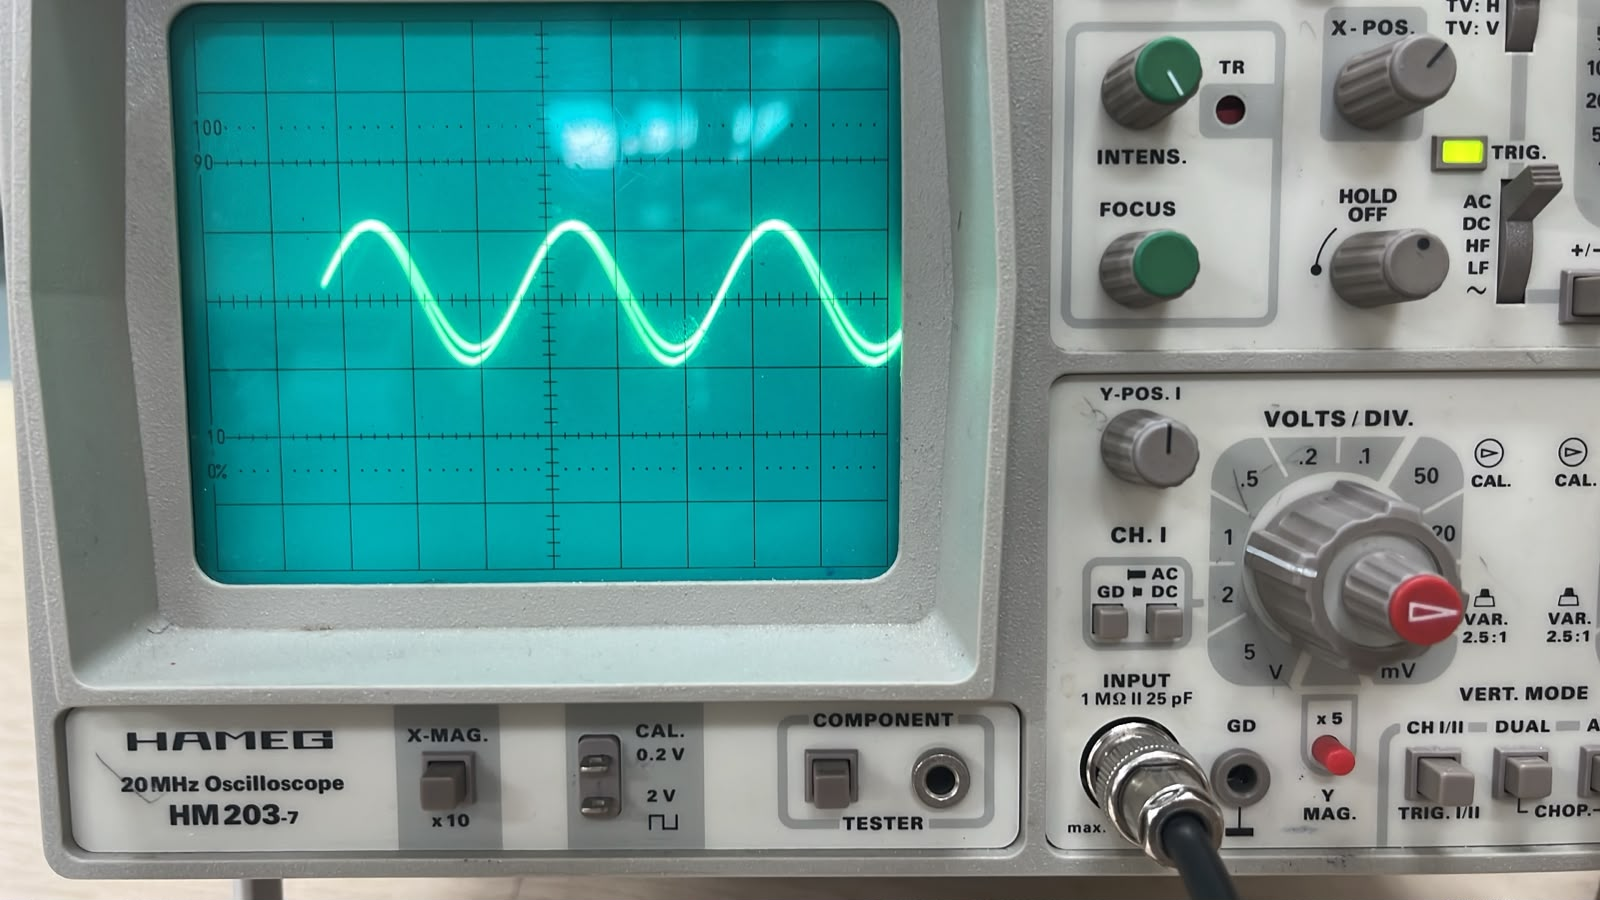
\includegraphics[width=\linewidth]{imagenes/rlc_pantalla.jpeg}
 \end{minipage}\hfill
 \begin{minipage}[t]{0.49\textwidth}
  \centering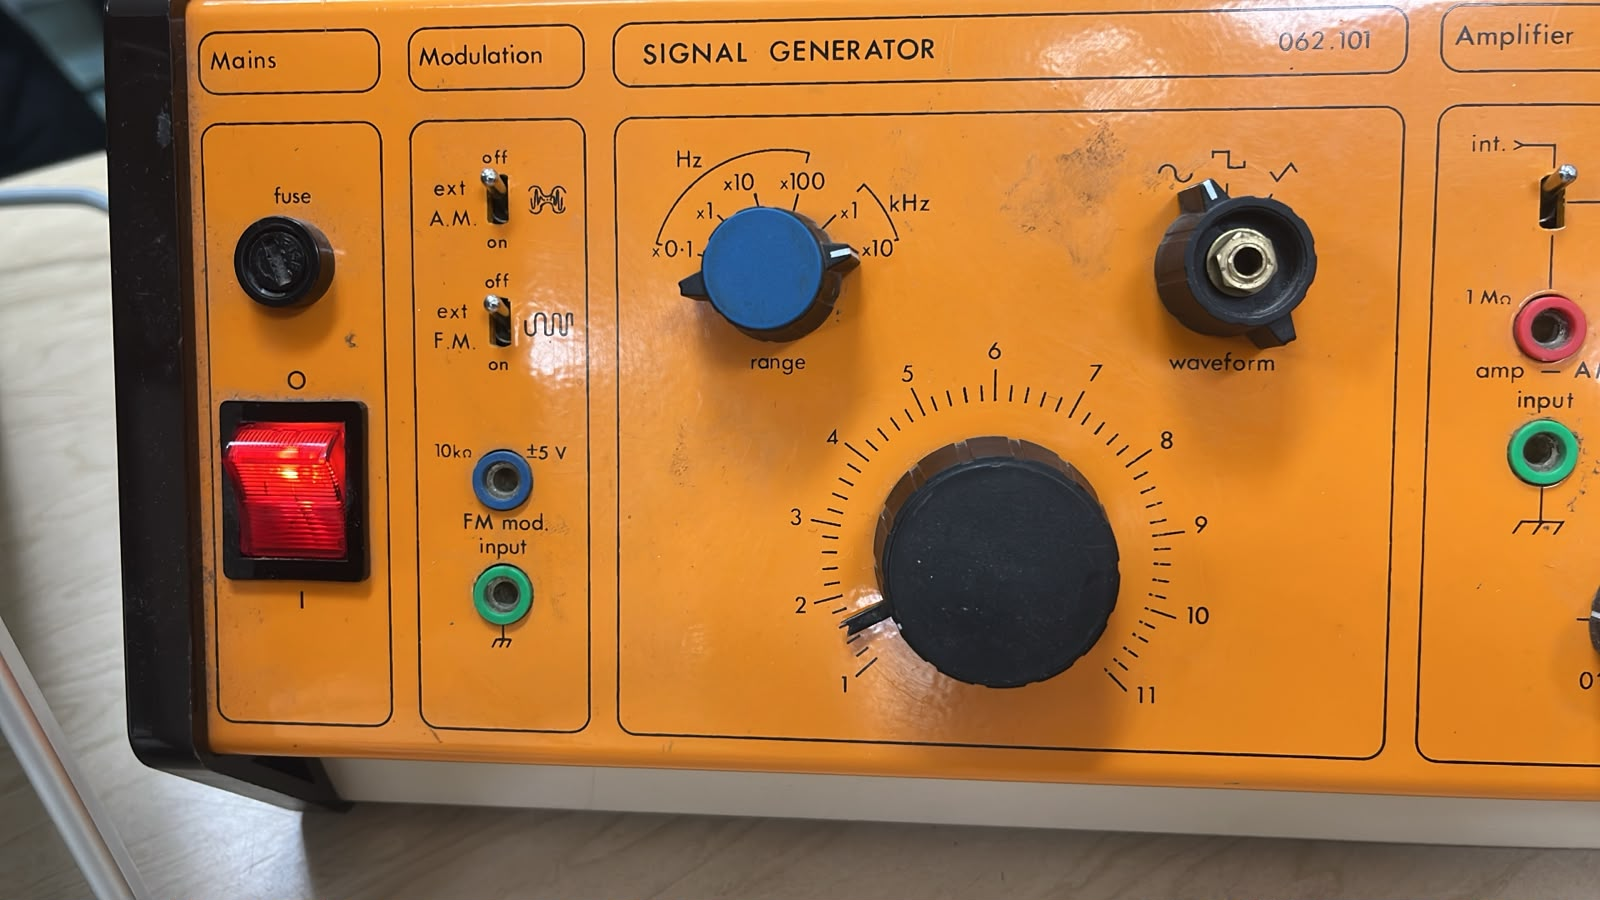
\includegraphics[width=\linewidth]{imagenes/rlc_frecuencia.jpeg}
 \end{minipage}
 \captionof{figure}{Registro cercano a la resonancia: señales del osciloscopio y ajuste aproximado del generador. La frecuencia se lee de un dial analógico y no de un frecuencímetro.}
 \label{fig:resonancia_fotos}
\end{center}
\begin{center}
 \begin{tikzpicture}
\begin{axis}[width=0.92\textwidth,height=6.2cm,xmin=1,xmax=50,ymin=-90,ymax=90,
 xlabel={$f$ (kHz)},ylabel={$\varphi_V$ (grados)},grid=major,ytick={-90,-45,0,45,90},
 tick label style={font=\small},label style={font=\small},
 legend style={font=\small,at={(0.98,0.05)},anchor=south east}]
 \addplot[udecazul,very thick,domain=1:50,samples=200]{atan((2*pi*x*\LRLC-1000000/(2*pi*x*\CRLC))/(1000*\RRLC))};
 \addlegendentry{Modelo RLC ideal}
 \addplot[gray,dashed] coordinates {(\FRes,-90) (\FRes,90)};
 \addlegendentry{$f_{r,\mathrm{teo}}\approx16{,}8$ kHz}
 \addplot[observado,densely dotted,thick] coordinates {(\FDial,-90) (\FDial,90)};
 \addlegendentry{Dial $\approx17$ kHz (orientativo)}
\end{axis}
\end{tikzpicture}

 \captionof{figure}{Curva teórica única de $\varphi_V$ frente a $f$ para el circuito RLC de la guía. El cruce por cero indica $f_r\approx\SI{16.8}{\kilo\hertz}$. La línea punteada señala la lectura orientativa del generador; no representa un barrido experimental.}
 \label{fig:fase_rlc}
\end{center}
\begin{center}
 \begingroup
\newcommand{\panelRLC}[3]{%
 \begin{scope}[shift={(#1,0)}]
  \pgfmathsetmacro{\ff}{#2*\FRes}
  \pgfmathsetmacro{\vl}{2*pi*\ff*\LRLC/(1000*\RRLC)}
  \pgfmathsetmacro{\vc}{1000/(2*pi*\ff*\CRLC*\RRLC)}
  \pgfmathsetmacro{\net}{\vl-\vc}
  \draw[-{Stealth[length=2mm]},gray] (0,0)--(1.3,0) node[right,font=\scriptsize] {$\widetilde I$};
  \draw[-{Stealth[length=2mm]},udecazul,thick] (0,0)--(1,0);
  \ifdim#2pt<1pt
   \node[above,font=\scriptsize,text=udecazul] at (0.45,0) {$\widetilde V_R$};
  \else
   \node[below,font=\scriptsize,text=udecazul] at (0.45,0) {$\widetilde V_R$};
  \fi
  \draw[-{Stealth[length=2mm]},udecazul,thick] (0,0)--(0,\vl) node[left,font=\scriptsize] {$\widetilde V_L$};
  \draw[-{Stealth[length=2mm]},udecazul,thick] (0,0)--(0,-\vc) node[left,font=\scriptsize] {$\widetilde V_C$};
  \draw[gray,densely dashed] (1,0)--(1,\net);
  \draw[-{Stealth[length=2mm]},observado,very thick] (0,0)--(1,\net);
  \node[above right,font=\scriptsize,text=observado] at (1,\net) {$\widetilde V_g$};
  \node[font=\small\bfseries] at (0.6,1.6) {#3};
  \node[font=\scriptsize] at (0.6,-1.6) {$f=\pgfmathprintnumber[fixed,precision=1,use comma]{\ff}$ kHz};
 \end{scope}}
\begin{tikzpicture}[x=1.7cm,y=1.3cm]
 \panelRLC{0}{0.8}{$f<f_r$}
 \panelRLC{3.25}{1}{$f=f_r$}
 \panelRLC{6.5}{1.2}{$f>f_r$}
\end{tikzpicture}
\endgroup

 \captionof{figure}{Fasores teóricos normalizados de RLC, con la corriente como referencia: comportamiento capacitivo por debajo de $f_r$, compensación de $\widetilde V_L$ y $\widetilde V_C$ en resonancia y comportamiento inductivo por encima de $f_r$.}
 \label{fig:fasores_rlc}
\end{center}

\subsection{Registro de voltajes}
\porcompletar{incorporar los voltajes del generador, resistor, condensador y bobina solo si existe un registro que permita conocer la escala vertical y su ajuste. Indicar si cada valor es pico, pico a pico o eficaz.}
% La guía solicita voltajes. No se inventan valores ni se deducen de escalas no verificadas.

\begin{multicols}{2}
\raggedcolumns
\section{Análisis}
\subsection{Comportamiento de RC y RL}
En RC, las estimaciones fueron \SI{86.7}{\degree}, \SI{89.5}{\degree} y \SI{50.9}{\degree}. Los valores a \SI{500}{\hertz} y \SI{1}{\kilo\hertz} permanecen próximos a \SI{90}{\degree}; la pequeña inversión entre ellos difiere de la disminución monótona ideal. A \SI{8}{\kilo\hertz}, el desfase disminuye claramente y coincide de cerca con el modelo. La mayor diferencia fue de aproximadamente \SI{5.2}{\degree}, a \SI{1}{\kilo\hertz}.

En RL, el retraso aumenta desde \SI{23.4}{\degree} hasta \SI{74.2}{\degree} al incrementar la frecuencia, de acuerdo con el crecimiento de $X_L$. Las diferencias con el modelo fueron aproximadamente \SI{3.9}{\degree}, \SI{-3.0}{\degree} y \SI{0.0}{\degree} al redondear a una décima. En conjunto, las seis estimaciones describen el comportamiento capacitivo e inductivo esperado.

\subsection{Lecturas y calibración}
No pudo verificarse la posición de CAL porque falta la tapa indicadora del ajuste fino de TIME/DIV. Como se mantuvo ese ajuste durante la experiencia, se examinó una corrección multiplicativa común; los períodos y las frecuencias nominales no permiten obtener un único factor consistente. Por ello, los tiempos se presentan con el supuesto de la ecuación~\eqref{eq:reconstruccion}. El desfase no depende de ese factor, ya que se cancela en $\Delta t/T$ \cite{manualhameg}.

Para RC a \SI{500}{\hertz} se utilizó el tramo continuo izquierdo de la primera prueba, que permite separar ambas señales y da cerca de \SI{87}{\degree}. La segunda prueba da cerca de \SI{100.5}{\degree}; se conserva como registro alternativo en el anexo. No se promedian ambas porque no ofrecen una lectura de fase consistente. A \SI{10}{\kilo\hertz} en RL, la separación es pequeña respecto del grosor de las trazas, por lo que la lectura es especialmente sensible.

\subsection{Condición de resonancia}
La lectura orientativa de \SI{17}{\kilo\hertz} está cerca de los \SI{16.8}{\kilo\hertz} nominales, y las señales muestran una proximidad de fase compatible con la búsqueda de resonancia. La tolerancia del condensador, el valor real de la inductancia, la resistencia de la bobina y la lectura del dial pueden modificar esa comparación. El registro disponible permite una evaluación cualitativa, pero no una determinación precisa de $f_r$ ni de su incertidumbre.

\section{Conclusiones}
Las fases reconstruidas de las fotografías reproducen el adelanto de la corriente previsto para RC y el retraso previsto para RL, suponiendo las conexiones de la guía y la ausencia de inversión de canal. En RC se observó una reducción marcada del desfase a \SI{8}{\kilo\hertz}; en RL, el retraso aumentó con la frecuencia. Las diferencias angulares respecto del modelo ideal fueron menores que aproximadamente \SI{6}{\degree} para las seis condiciones seleccionadas.

En RLC, el valor nominal de resonancia fue \SI{16.8}{\kilo\hertz}, cercano al ajuste orientativo de \SI{17}{\kilo\hertz} fotografiado. La coincidencia aproximada de fase apoya la identificación de una condición próxima a la resonancia. Los tiempos dependen de las frecuencias nominales utilizadas como supuesto, mientras que los ángulos proceden del cociente entre distancias de las señales.

\bibliographystyle{apalike}
\bibliography{Referencias}
\end{multicols}

\clearpage
\appendix
\section{Lecturas utilizadas y trazabilidad}
La tabla~\ref{tab:lecturas} conserva las distancias estimadas de la pantalla y las lecturas nominales del selector. Estas últimas son distintas de los factores efectivos reconstruidos de las tablas principales. La identificación de corriente adelantada o retrasada supone CH1 conectado a $v_g$, CH2 a $v_R$, INV desactivado y el montaje indicado.
\begin{table}[htbp]
\centering
\small
\setlength{\tabcolsep}{6pt}
\caption{Entradas utilizadas: distancias fotográficas y selector nominal de tiempo, sin confirmar CAL.}
\label{tab:lecturas}
\begin{tabular}{cccccc}
\toprule
Circuito & $f$ (Hz) & $\Delta h$ (div) & $H$ (div) & TIME/DIV nominal & Prueba \\
\midrule
RC & 500 & \num{0.465} & \num{1.93} & \SI{1}{\milli\second\per\division} & 1 \\
RC & 1000 & \num{0.41} & \num{1.65} & \SI{0.5}{\milli\second\per\division} & 2 \\
RC & 8000 & \num{0.38} & \num{2.69} & \SI{20}{\micro\second\per\division} & 2 \\
RL & 10000 & \num{0.10} & \num{1.54} & \SI{20}{\micro\second\per\division} & 2 \\
RL & 50000 & \num{0.31} & \num{1.94} & \SI{5}{\micro\second\per\division} & 2 \\
RL & 100000 & \num{0.20} & \num{0.97} & \SI{5}{\micro\second\per\division} & 2 \\
\bottomrule
\end{tabular}
\end{table}


\textbf{Registro alternativo de RC a \SI{500}{\hertz}.} En la segunda prueba se estimó $\Delta h=\num{1.10}$ div, $H=\num{3.94}$ div y un selector de \SI{0.5}{\milli\second\per\division}, que dan $|\Delta\varphi|\approx\SI{100.5}{\degree}$. La primera prueba se midió en el tramo izquierdo continuo; variar la longitud de ese tramo dio aproximadamente \SI{86.7}{\degree} a \SI{86.9}{\degree}, antes del redondeo. Ese rango describe la estabilidad de la lectura fotográfica y no una incertidumbre instrumental.

\begin{center}
 \begin{minipage}[t]{0.47\textwidth}
  \centering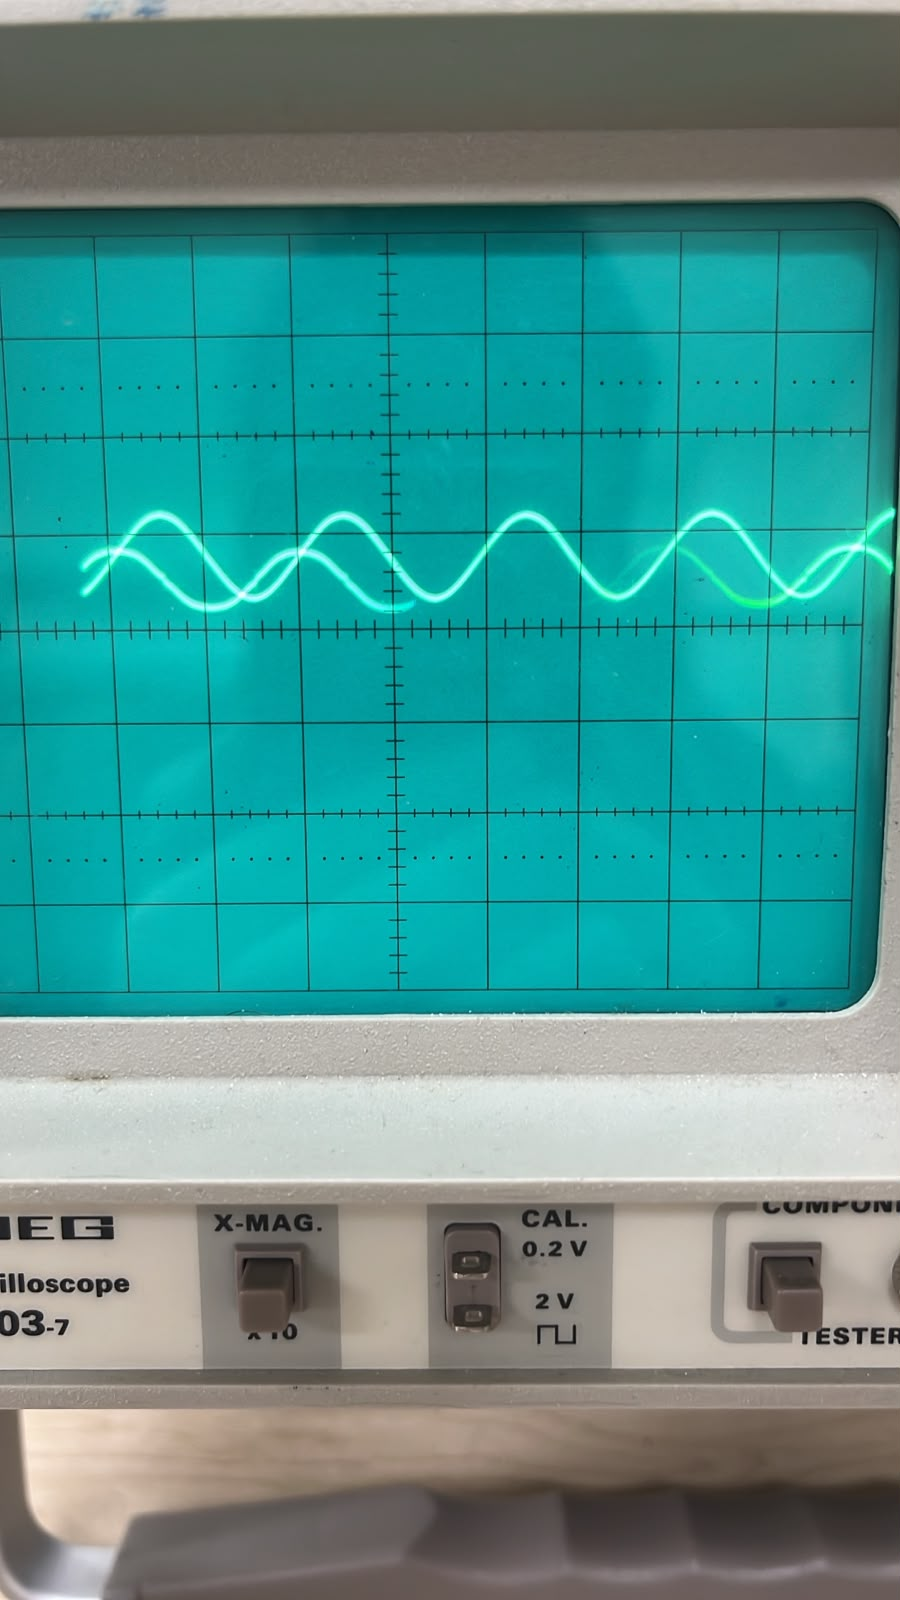
\includegraphics[height=6.8cm,keepaspectratio]{imagenes/rc_500_grafica.jpeg}
  \par\small Primera prueba: usada para la tabla.
 \end{minipage}\hfill
 \begin{minipage}[t]{0.49\textwidth}
  \centering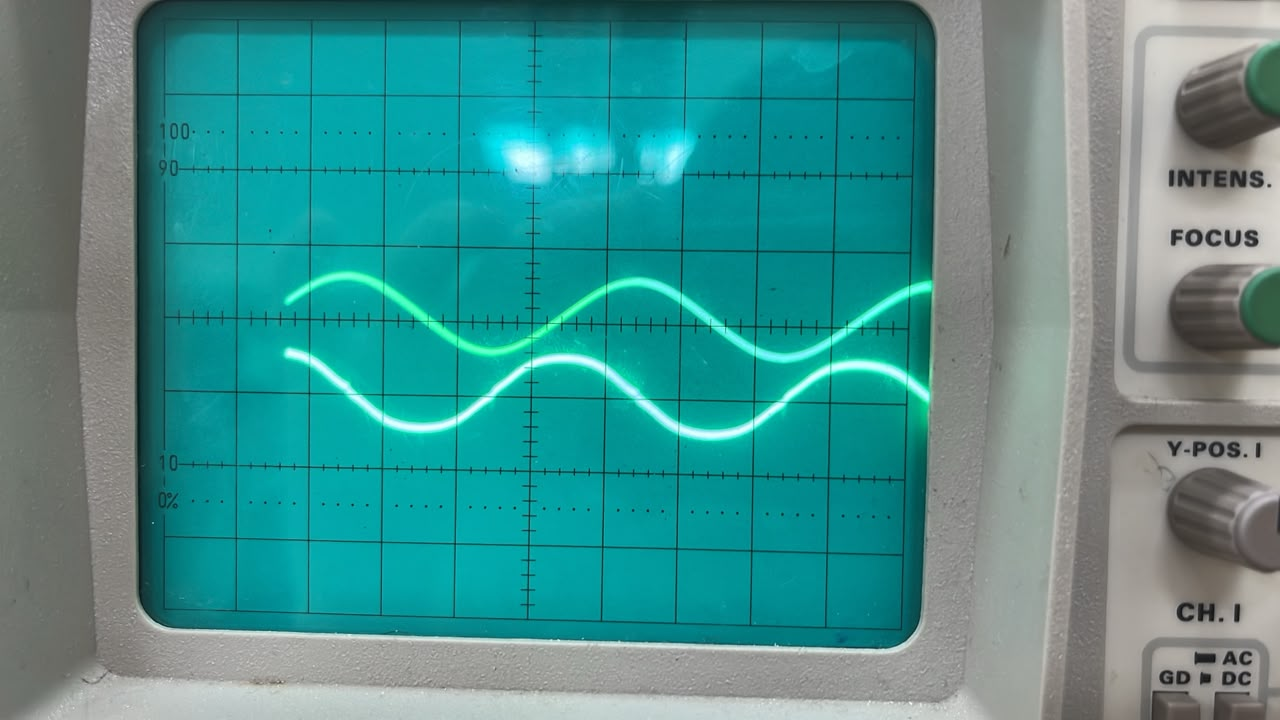
\includegraphics[width=\linewidth]{imagenes/rc_500_alternativa.jpeg}
  \par\small Segunda prueba: registro alternativo.
 \end{minipage}
 \captionof{figure}{Registros de RC a \SI{500}{\hertz}. Se mantienen ambas fotografías para distinguir la lectura elegida del registro alternativo.}
\end{center}
Los archivos fuente de todas las filas se incluyen en la carpeta \texttt{imagenes/}; la correspondencia de nombres se encuentra en \texttt{datos/fuentes.csv}. Los dígitos presentados y el redondeo de las tablas no deben interpretarse como una especificación de exactitud del instrumento.
\end{document}
